\documentclass[11pt,letterpaper]{report}
\usepackage[spanish]{babel}
\usepackage[utf8]{inputenc}

\usepackage{multirow}
\usepackage{subfigure}
\usepackage{algorithm}
\usepackage{algorithmic}
\usepackage{listings}
\usepackage{amsthm}
\usepackage{textcomp}
\usepackage{multicol}
\usepackage{float}
\usepackage{url}
\usepackage{color}
\usepackage{xcolor}
\usepackage{enumerate}
\usepackage{enumitem}
\usepackage{newlfont}
\usepackage{psfrag}
\usepackage{charter}
\usepackage{setspace}
\usepackage{longtable}
\usepackage{subfigure}
\usepackage{tabularx}
\usepackage[pdftex]{graphicx}
\usepackage[centertags]{amsmath}
\usepackage{newlfont}
\usepackage{psfrag}
\usepackage{amsfonts}
\usepackage{amssymb}
\usepackage{framed}
\usepackage{listings}
\usepackage{icomma}
\usepackage{epstopdf}
\usepackage{UTFSM_Tesis}
\usepackage[active]{srcltx}
\usepackage[unicode]{hyperref}

\hfuzz2pt
%\setlist[itemize]{noitemsep, topsep=0pt}
\setlist[itemize]{itemsep=1pt, topsep=0pt}

\hypersetup{%
pdftitle={Memoria ivillacu},
pdfauthor={Ignacio Javier Villacura de la Paz},
pdfkeywords={memoria, ivillacu},
bookmarksnumbered,
pdfstartview={FitH},
urlcolor=cyan,
}%

\hyphenpenalty=5000
\tolerance=1000
\hyphenation{no-me-cor-tes}
\oddsidemargin  0cm    % Ancho Legal 21,59cm
\evensidemargin 0.5cm  % Alto  Legal 35,56cm
\textwidth      16.5cm
\topmargin       -1.5cm
%\voffset        2cm  % Margen superior
\textheight     22cm
%\parindent      1cm
\parskip        2ex

\newlength{\defbaselineskip}
\setlength{\defbaselineskip}{\baselineskip}

\newcommand{\setlinespacing}[1]%
           {\setlength{\baselineskip}{#1 \defbaselineskip}}
% \newcommand{\doublespacing}{\setlength{\baselineskip}%
%                            {1.3 \defbaselineskip}}
% \newcommand{\singlespacing}{\setlength{\baselineskip}{\defbaselineskip}}

%Formulas matem?ticas utilizadas en el paper
\newcommand{\bbbr}{\mathbb R}

\newcounter{defcount}
\setcounter{defcount}{0}
\newenvironment{definition}[1]
%%\bf\normalsize
{% This is the begin code \bf
\stepcounter{defcount}{\noindent \bf \normalsize Definition \bf \arabic{defcount}: #1}\nopagebreak[3] \\
\begin{it}
}
{% This is the end code
\end{it}

}

\newcounter{defcount1}
\setcounter{defcount1}{0}
\newenvironment{property}[1]
%%\bf\normalsize
{% This is the begin code \bf
\stepcounter{defcount1}{\noindent \bf \normalsize Property \bf \arabic{defcount1}: #1}\nopagebreak[3] \\
\begin{it}
}
{% This is the end code
\end{it}
}

%Redefine plain page style
% \fancypagestyle{plain}{
% \fancyhf{}
% \renewcommand{\headrulewidth}{0pt}
% \fancyfoot[LE,RO]{\thepage}
% }
%
% % Code for creating empty pages
% % No headers on empty pages before new chapter
% \makeatletter
% \def\cleardoublepage{\clearpage\if@twoside \ifodd\c@page\else
%     \hbox{}
%     \thispagestyle{plain}
%     \newpage|||
%     \if@twocolumn\hbox{}\newpage\fi\fi\fi}
% \makeatother \clearpage{\pagestyle{plain}\cleardoublepage}
%
% % Define pagestyle
% \pagestyle{    fancy}
% \fancyhf{}
% \renewcommand{\chaptermark}[1]{\markboth{ \emph{#1}}{}}
% \fancyhead[LO]{}
% \fancyhead[RE]{\leftmark}
% \fancyfoot[LE,RO]{\thepage}

%U1 hasta olympiaCentrodecompras
% tomar micro 60 en el paradero del mall, 3 paraderos mas al norte, himmel.

\setlength\parindent{0pt}

\setcounter{secnumdepth}{5}
\setcounter{tocdepth}{5}

% Colores
\newcommand{\blue}{\textcolor{blue}}
\newcommand{\red}{\textcolor{red}}
\newcommand{\green}{\textcolor{green}}

% Comentarios
\newcommand{\cmf}{\textcolor{red}{CMF:}\textcolor{blue}}
\newcommand{\GAM}{\emph{Gamification}}
\newcommand{\gam}{\emph{gamification}}

% Cambiar "Bibliography" a "Bibliografía"
\renewcommand{\bibname}{Bibliografía}

\begin{document}

% Agregué un \\ para que se veira mejor el título en la portada
\title{Evaluación estratégica del uso\\ de Gamification en ventas \emph{on-line}}
\author{Ignacio Javier Villacura de la Paz}
\submitdate{Marzo - 2015}
\copyrightyear{2015}
\ingciv
\profguia{Dr. Horst von Brand}
\profcorr{M.Sc. Cecilia Reyes}
\dedicate{
Agradecimientos
}

\nolistoffigures
\nolistoftables
\beforepreface
%  \listoftables
%  \listoffigures
%  \listofalgorithms
%\input{agradecimientos.tex}
El problema que poseen las pequeñas empresas contra las empresas de mayor tamaño es interesante. Esto es debido
a que son las PyMe las que entregan la mayor parte del empleo en Chile. Desde que las multinacionales ingresaron
al país las pequeña empresa ha ido perdiendo terreno y desapareciendo y con ello a llevado a una mayor tasa de 
desempleo.
Este trabajo de memoria se enfoca en la diferencia que existe entre estas empresas en lo que a ventas \emph{on-line}
se refiere. Este es un sector en el cual se puede competir de igual a igual pero se necesita una gran cantidad de 
recursos que una pequeña empresa no posee, desde capital a conocimiento. 
Para ayudar a acortar esta diferencia en el sector de ventas \emph{on-line} se utilizara {\gam} como herramienta para
atraer a nuevos clientes y retenerlos con el objetivos de que se incentiven en volver a comprar en la tienda virtual. 
Eso se hará implementando un sistema web que contempla la tienda virtual y módulos que interactúan con el cliente 
y así mostrar las ideas que nos presenta {\gam}. Además, para apoyar la implementación del sistema se desarrollo
una encuesta que tiene como objetivo ver el conocimiento de la población sobre {\gam}, la interacción diaria con el 
concepto de {\gam} y obtener los beneficios que mas atraen a los clientes.
Luego de la implementación de la tienda virtual, esta tuvo una pobre recepción del publico debido a factores
externos al sistema como son la falta de interés por parte de la empresa y problemas económicos. De la encuesta
realizada se obtuvo que a la población le interesa el uso {\gam} por parte de las empresas debido a que estos
entregan beneficios y es esto lo que atrae y retiene a los clientes. Un punto importante es lo necesario
de buscar una nueva forma de entrega de beneficios debido a que la acumulación de puntos ya no es un sistema 
interesante para el publico.
Finalmente, se puede destacar que el uso de {\gam} ayuda a las empresas a mejorar sus ventas debido a que al 
cliente le interesa una forma de obtener beneficios al momento de comprar en alguna tienda. Con esto se puede
competir mas directamente con empresas de mayor tamaño.

Keywords: \textbf{\emph{Gamification}, \emph{E-commerce}, \emph{Wordpress}, Sistemas Web}

\afterpreface
\onehalfspacing

\chapter{Introducción}
\label{ch:introduccion}
    La diferencia en el mercado de ventas electrónica ha sido demostrada por la gran
brecha que existe entre las micro, pequeñas o grandes empresas, sobre todo con el
pasar del tiempo, donde la tecnología ha llegado a ser un actor principal
tanto en el marketing, ventas y en el manejo interno de cada institución.

Al no poder competir con las grandes empresas, las micro o pequeñas empresas se ven
limitadas a tener un ámbito reducido y netamente local, sin poder establecer
una expansión tan favorable, lo que hace que las ventas se estanquen.

Desde el comienzo de la masificación del uso de Internet, dicha brecha se ha
visto reducida, por tres factores: (1) La cantidad de clientes \emph{online}
y su crecimiento exponencial, (2) Micro, pequeñas y grandes empresas con capacidad
de acceder al mismo contenido en Internet, por lo que se desarrollaba una competencia
más justa, y (3) Las ventas ya no estaban limitadas a un conjunto de clientes
cercanos a la tienda física.

Actualmente, diversos sistemas son ampliamente utilizados en la creación
de tiendas virtuales, de los que podemos destacar:

\begin{itemize}
    \item {\bf Magento}~\footnote{http://www.magento.com}:
        Plataforma stand-alone OpenSource que es utilizada para crear tiendas online
        de mediana a alta escala.
        Esta compañía fue comprada por eBay pocos años luego de su lanzamiento.

    \item {\bf Wordpress $+$ Woocommerce}~\footnote{http://www.woocommerce.com}:
        Creado como un plugin del reconocido CMS Wordpress, su fácil configuración
        y mantención lo hacen ser utilizado por micro o pequeñas empresas hasta
        grandes multinacionales como Cosmopolitan.

    \item {\bf Prestashop}~\footnote{http://www.prestashop.com}:
        Solución OpenSource para tiendas online no tan conocida en la actualidad
        pero ha crecido en uso en los últimos años.
        Su gran catalogo de traducciones la hace ser utilizada en todo el mundo.

\end{itemize}

Adicionalmente, la investigación y el desarrollo de técnicas asociadas a ampliar
y mantener la clientela ha sido un factor clave en el desarrollo de las empresas,
de las cuales se destaca {\GAM}, tema principal de la presente memoria.

La idea central de  {\GAM} es poder utilizar elementos del diseño de juegos
para mantener la atención del consumidor, manteniendo una frecuencia de compras,
para así obtener beneficios en el futuro.

En el presente trabajo, combinaremos un sistema de ventas online, concentrándonos
en proveer un sistema de fácil uso y administración, aplicando la técnica {\GAM}
para ayudar a micro o pequeñas empresas a surgir.

El objetivo principal de la memoria es:

\begin{itemize}
    \item Evaluar el impacto de {\GAM} en ventas de videojuegos online.
\end{itemize}

Los objetivos específicos de la memoria son:
\begin{itemize}
    \item Selección de plataforma e-commerce.
    \item Creación de herramientas, utilizando {\GAM}, que apoyen la
          venta online de videojuegos.
    \item Desarrollo de módulo que unifique las herramientas creadas para sistema
          seleccionado.
    \item Proponer métricas para el análisis del uso de {\GAM}.
    \item Análisis de los datos preliminares obtenidos.
\end{itemize}

\cmf{(Soluciona esto al final de todo)
Esta sección por lo general es un párrafo, que explica en 1 o 2 frases lo que
hay en cada capítulo, no con tanto detalle como lo hiciste. Lo unico que hice
fue cambiar el formato a como se explican las cosas, pero no resumi ni modifique
el contenido de cada capitulo que habias escrito. Quizas ver otras memorias
seria bueno}.

El presente documento se encuentra organizado de la siguiente forma.
En la primera parte del capítulo~\ref{ch:gamification} se expone la historia tras
el concepto, los distintos estereotipos de jugadores que existen y algunos ejemplos
de empresas que han utilizado \emph{gamification} a nivel mundial.
En la segunda parte se explica la definicion de este concepto y se realiza un
desglose de esta para explicar cada una de las ideas que lo definen.
Luego se exponen contextos en donde es utilizada con exito \emph{gamification}
y por ultimo las criticas que se le han hecho a la utilizacion de esta idea.

En el capítulo~\ref{ch:desc} se da la explicación del problema a enfrentar
y dar solución.
Tambien se da una descripcion de los datos asociados como la tienda a la cual se
le implementara la solucion y tambien la información para entender el contexto
de ventas online de micro y pequeñas empresas.

A continuación, en el capítulo~\ref{ch:solucion} se da a concer la solucion
propuesta para enfrentar el problema.
La primera parte se expone la metodologia pensada para la solucion como son el
sistema base y los plugins necesarios para implementar de buena forma la solucion.
En la segunda parte se explican todas las herramientas a utilizar y cual es su
rol en esta.
Tambien se explica la utilizacion de la encuesta evualativa creada para obtener
informacion mas directa de los posibles clientes.

El estudio experimental es abordado en el capítulo~\ref{ch:estudio} donde
se explican los resultados obtenidos en las dos formas de captura de datos,
sistema web y encuesta.
En el sistema web se muestra la compracion entre un sistema sin la implementacion
de la solucion y otra con esta.
Por parte de la encuesta se desglosa y se explican los datos obtenidos en cada
una de las preguntas.

Por último en el capítulo~\ref{ch:conclusiones} se exponen las conclusiones
obtenidas luego de la implementación de la solucion y del comportamiento de esta
con el los usuarios.


\chapter{Gamification}
\label{ch:gamification}
    \section{Historia}

El término {\GAM} fue acuñado cerca del año 2008\cite{DefineGamefication}.
El objetivo fue crear un término que agrupara todas las ideas y elementos
utilizados en el diseño de juegos que pudiesen ser utilizados en otros contextos
(distintos a los de entretención).
En el año 2010, este término llega a ser conocido mundialmente ya que logra
aparecer en los \emph{trend} en google\cite{LiCap1.3}, palabras mas buscadas
del año.

\begin{figure}[!htb]
  \centering
  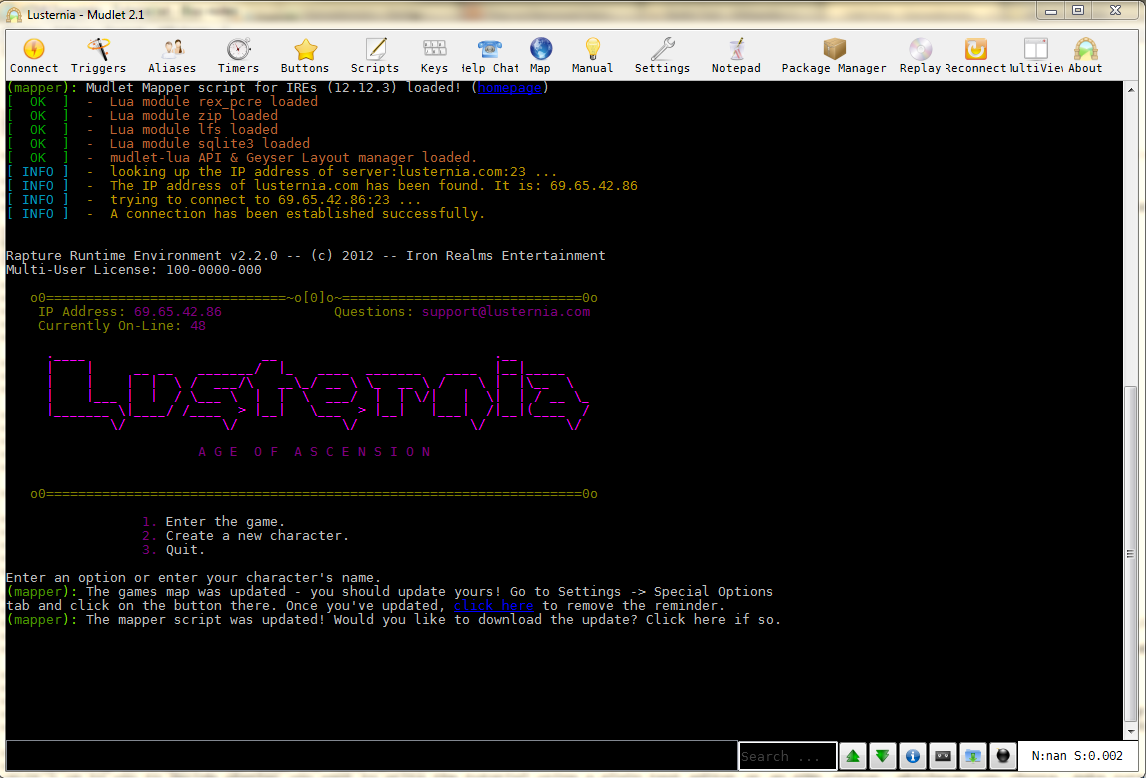
\includegraphics[width=0.8\textwidth]{images/mudclient.png}
  \caption[Caption for LOF]{\red{CAMBIAR CAPTION}}
  \label{fig:MudClient}
\end{figure}

El concepto básico fue inicialmente utilizado en la década de los ochenta con el
objetivo de mejorar y actualizar el juego llamado \emph{MUD}\ref{fig:MudClient},
\emph{Multy User Dungeons}.
El desarrollador, Richard Bartle, comenzó un análisis basado en los jugadores
donde encontró 4 estereotipos \ref{fig:Players}.

\begin{itemize}
    \item \emph{Achievers}:
        Jugadores que se enfocan en obtener éxito mediante la obtención de puntos,
        premios, u otra forma de demostrar el trabajo puesto en el juego.
        Estos tipos de jugadores se esfuerzan la mayoría del tiempo en la obtención
        de dicho prestigio, lo que conlleva a casi una nula ventaja en la
        jugabilidad o avance en el juego.

    \item \emph{Explorers}:
        A estos jugadores les gusta explorar el mundo en el cual están inmersos,
        mas allá de lo geográfico, les interesan detalles dificiles de encontrar o
	caracteristicas escondidas del juego.
        La pasión detrás del conocer cada rincón del universo del juego los lleva 
        a experimentar la mayor cantidad de casos y con esto logran conocer mejor
        el juego, mas alla de los propios desarrolladores.
        Un ejemplo de \emph{explorers} son jugadores solitarios, que buscan el
        poder descubrir lugares nuevos, aventurándose en el mundo del juego.

    \item \emph{Killers}:
        Este tipo de jugadores son los más competitivos, pues buscan destacarse
        dentro de los usuarios, creando drama entre otros jugadores.
        Algunos ejemplos de este tipo de jugadores son los \emph{Trolls},
        \emph{Hackers}, \emph{Cheaters}, etc.
        Pero no existen sólo aspectos negativos en éste tipo de jugadores,
        pues las personas que se dedican a un juego de forma profesional
        suelen apreciar la competitividad.

    \item \emph{Socializers}:
        Personas que son atraídas por la parte social de los juegos,
        en desmedro de la estrategia u otras partes de este.
        Se puede decir que estos jugadores son el ``Corazón'' del juego,
        pues ponen las relaciones interpersonales como la primera prioridad
        del juego en el que están inmersos.
        Los jugadores \emph{Socializers} consideran el juego
        como un vehículo para generar nuevas relaciones de amistad, y llevan
        sus grupos de juego, con los que comparten aventuras, al mundo real.

\end{itemize}

\begin{figure}[!htb]
  \centering
  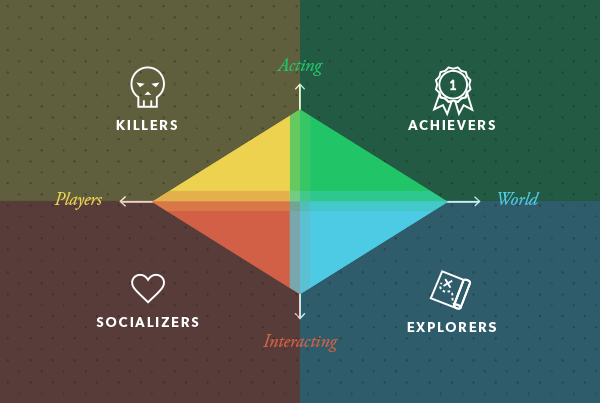
\includegraphics[width=0.8\textwidth]{images/TypeOfPlayersBartle.png}
  \caption[Caption for LOF]{Real caption\footnotemark}
  \label{fig:Players}
\end{figure}


Con esta información, el desarrollador modificó el juego para satisfacer cada
tipo de jugador.
Este cambio tuvo un gran éxito y demostró una nueva forma de atraer a diferentes
tipos de jugadores a un juego en particular, esto llamo la atención de empresas
que vieron este concepto como una nueva forma de atraer y retener a sus clientes.

Diversas compañías actualmente usan {\GAM}, varias han creado plataformas para
aplicar sus principios y estrategias.
En $2007$, la compañía \emph{Bunchball}\footnote{www.bunchball.com} fue una de
las primeras en implementar y proveer una plataforma gamificada como un
servicio\cite{Gam:Bunchball:1}.
\emph{Bunchball} tuvo clientes de gran tamaño como Bravo\footnote{www.bravotv.com}
y \emph{The USA network}\footnote{www.usanetwork.com}\cite{Gam:Bunchball:2},
lo que significó el éxito del modelo adaptado para su plataforma web.

Otras grandes empresas que utilizan {\GAM} en la actualidad son:
SAP AG, IBM, EMC, CA, Slalom Consulting, Deloitte, Microsoft, LiveOps,
RedCritter\cite{Gam:Companies:1}, etc.

Debido al peso que {\GAM} fue tomando dentro del mundo,
se crearon eventos para discutir sobre experiencias de éxito e ideas para
el futuro, como lo fue \emph{Gamification 2013},
un evento de discusión sobre su futuro\cite{Gam:Events:1}.
En $2014$ se llevará a cabo \emph{Loyalty Gamification World Championship}
en San Francisco, USA\cite{Gam:Events:2}.

\section{Definición}

Hoy en día {\GAM} se ha convertido en una herramienta para las empresas
para poder captar mas clientes.
Cada día aumenta el uso de este concepto por lo que es necesario entregar una
definición apropiada para el concepto.
{\GAM} se puede definir como ``el uso de elementos del diseño de juego en contextos
diferentes al de entretención''.
Para entender mejor los conceptos bajo esta definición se explicaran por partes:

\begin{itemize}
    \item {\bf Juego:}
        En primer lugar este concepto se refiere al juego en su totalidad,
        y no a la acción de jugar.
        Este concepto es caracterizado por un conjunto de reglas explícitas,
        que crean un ambiente en donde los jugadores buscan la competición para
        completar objetivos y metas.

    \item {\bf Elementos del diseño de juego}:
        Dentro de este concepto se puede encontrar 2 definiciones.
        La primera, es una definición estricta que sólo acepta ciertos elementos
        únicos.
        La segunda, es una definición en donde todos los elementos pueden ser
        utilizados.
        Para llegar a una definición robusta es necesario juntar ambas y así
        obtener un conjunto mas restrictivo en donde los elementos a utilizar
        son característicos a los juegos, que se encuentran en la mayoría de estos
        y que cumplen una rol importante en la jugabilidad de estos.

    \item {\bf Contextos diferentes al de juego:}
        Este es el concepto mas complejo de explicar debido a que es una idea
        abstracta.
        Una forma de explicarla es como una situación de la vida cotidiana
        que existe fuera de un juego o de un ambiente que contiene {\GAM}.

\end{itemize}

\section{Utilización}

Esta técnica a sido utilizada en diferentes áreas y contextos en todo el mundo,
del cual el Marketing ha sido una de las áreas más beneficiada con su
implementación.
Mas de 70 empresas en el ranking de \emph{Forbes Global $2000$} han utilizado o
piensan hacerlo con el motivo de una nueva fuente de marketing y como retención
de clientes\cite{Gam:Util:1}.
Un ejemplo exitoso del uso en marketing es \emph{Nike} con su aplicación
\emph{Nike+ Fuelband} que fue fue lanzada en enero del 2012\cite{Gam:Util:2}.
Con esta aplicación se logró crear un sistema gamificado en el cual se ayudaba
a sus clientes a mantener su estado física.
Otra empresa multinacional que a utilizado {\GAM} en marketing es \emph{McDonals}
con el uso de mecánicas de juego derivadas del juego de mesa \emph{Monopoly}.
Esta idea viene se viene implementando desde $1987$, por lo que al año $2010$
\emph{Mcdonals} incrementó sus ventas en los Estados Unidos en $5.6\%$
\cite{Gam:Util:2}.

{\GAM} también es utilizado como una herramienta para atraer y retener clientes,
adicionalmente es utilizado para alentar el correcto uso de un sitio web,
donde sitios web como StackOverflow y Samsung se aseguran de un sistema
de ranking por cada usuario y así establecer cierta fidelidad en respuestas
o reseñas.
StackOverflow, es una web dedicada a preguntas y respuestas sobre tecnología,
la cual entrega puntos  y logros a los usuarios al hacer determinadas tareas
de forma correcta.
Existen diferentes tipos de medallas y a medida  de que el usuario va ganando
puntos y reputación va obteniendo privilegios, siendo el mayor de estos ayudar a
moderar el sitio.
Samsung por su parte, también utiliza puntos y logros en su web pero esta
es enfocada a que los usuarios tengan interacción con la comunidad a nivel de
reseñas de productos y así crear contenido para la empresa\cite{Gam:Util:3}.

Educación y entrenamiento han sido otras áreas en donde a existido interés por
utilizar {\GAM}.
En los Estados Unidos, el departamento de educación de la ciudad de Nueva York
con el apoyo de \emph{MacArthur Foundation} y \emph{Bill and Melinda Gates
Foundation} crearon una escuela  llamada \emph{Quest to Learn}.
Lo que busca la escuela, es la modificación del sistema de aprendizaje,
utilizando mecanismos de juegos para así presentar la etapa de aprender
como algo mucho más llamativo para niños modernos\cite{Gam:Util:4}.

Otro sitio de educación utilizando esta técnica es \emph{Coursera},
compañía que se apoya de universidades de todo el mundo para enseñar
cursos sobre nuevos temas y tecnologías de manera gratuita vía e-learning.
La utilización de {\GAM} se ve reflejada en las medallas y certificados dados
a los estudiante, a medida que van completando tareas dentro del curso
hasta finalizarlo.
Dentro de todos los cursos dictados el mas popular es el de {\GAM}\cite{Gam:Util:5}.
En el año 2014, se inicio un proyecto llamado \emph{the True Life Game project}
que tiene como objetivo investigar las mejores formas de aplicar esta técnica en
la vida cotidiana.

Esta técnica también se usa en muchos otros ámbitos, pero en menor cantidad,
como productividad, autenticación, servicios financieros, entre otros.

\section{Criticas}

La idea de {\GAM}, desde sus inicios, a creado expectativas altas en todo el mundo
ya que ha sido utilizada por varias compañías, desde micro o pequeñas empresas
hasta multinacionales.
Pero existen retractores a la utilización de esta idea en la vida cotidiana.
Sebastian Detering, investigador de la universidad de Hamburgo, ha dicho que las
características mas utilizadas no son divertidas y crean una sensación falsa de
logro\cite{Gam:Crit:1}.
A esto se a sumado personas relacionadas con el diseño de juegos como son
Jon Radoff y Margaret Robertson,  que declaran que la utilización de {\GAM}
excluye otras partes del diseño como son la historia, las experiencias de juego
y que lo utilizado en este concepto es de lo mas básico, faltando mecánicas de
juego\cite{Gam:Crit:2}.

En el año 2012, la empresa analista \emph{Gartner} entregó un
reporte\cite{Gam:Crit:3} en el cual explicaba que la idea de {\GAM}
"basaba su éxito en la nobleza del usuario y de las altas expectativas
de las empresas por utilizar esta idea".
También se esperaba de que para el año 2014 el 80\% de las aplicaciones
gamificadas fallarían debido a una falta de buen diseño,
esto producido por la falta de seriedad al crear las aplicaciones,
así como, el intento de copiar e implementar esto a la mayoría de las ideas.


\chapter{Descripción del problema}
\label{ch:desc}
    \section{Descripción del problema}

Desde el nacimiento del comercio electronico ha existido una gran diferencia
entre las micro y pequeñas empresas con aquellas empresas con mayores recursos,
vease la figura \ref{tab:tam_empresa} que muestra las diferentes clasificaciones
de empresas existentes en chile.

\begin{table}[h]
\centering
\begin{tabular}{lrrr}
{\bf Empresa}  & {\bf Número de Trabajadores} & {\bf Porcentaje de ocupación} & {\bf Ventas anuales}\\
Micro    & 1 a 4                & 44.4\%  & menos de 2400 UF\\
Pequeña  & 5 a 49               & 37\%  & 2401 a 25000 UF\\
Mediana  & 50 a 199             & 13\%  & 25001 a 100000 UF\\
Grande   & más de 199           & 10\%  & más de 100000 UF\\
\end{tabular}
\caption[TamañoEmpresa]{Tamaño de empresa segùn cantidad de empleados y
la cantidad de estas en el mercado (SOFOFA Chile - \url{http://www.sofofa.cl/}).}
\label{tab:tam_empresa}
\end{table}


La problemática nace cuando la pequeña empresa desea desea utilizar el comercio
electrónico y no cuenta con los recursos necesarios, monetarios y humanos,
para lograr utilizar esta herramienta con éxito.

Esta situación es aprovechada por las grandes empresas para atraer y retener a los
clientes con un mayor marketing de productos disminuyendo las ventas de las
empresas pequeñas en donde muchas de estas terminan cerrando después de un cierto
tiempo.

Hoy en día las micro y pequeñas empresas tienen acceso a un sin número de
tecnologías que ayudan a la creación y administración de una tienda virtual.
Estas herramientas son cada vez mas fáciles de administrar por una persona
con conocimientos básicos debido principalmente a que sus curvas de aprendizaje
son menores que en años anteriores.

La problemática mayor es como incrementar la base de clientes de forma estable
para evitar fluctuaciones en la ventas y así poder tener una estabilidad económica.
Esta es la base del problema que se quiere resolver debido a que los negocios
pequeños tienen una falta de marketing online y no tienen exposición al público
objetivo.

La falta de exposición complica a que éstos negocios puedan atraer nuevos clientes
para poder aumentar las ventas.
Luego, si se logra entregar buen marketing a la micro o pequeña empresa y su
exposición en el mercado objetivo aumenta, existe otra arista de este problema
que es la retención de clientes, para así tener una estabilidad en el tema
de ventas, asegurando la permanencia en el tiempo.

La solución a este problema es de una alta complejidad, ya que se debe enfocar en
los clientes.
Estos son diferentes tipos de personas y por lo tanto la diversidad de gustos es
alta.

Si bien la dificultad de atraer a esta cantidad de distintos tipos de personas
es bastante alta, se puede enfocar en distintos grupos y así por cada segmento
de clientes, complacer gustos por separado.
{\GAM} cumple con esta forma de enfrentar la problemática teniendo elementos que
atraen varios tipos de clientes.

Para dar solución a esta problemática, se utilizarán aplicaciones gratuitas y de
bajo costo monetario. La base del sistema, wordpress, el plugin de comercio
electrónico, woocommerce, y el tema visual, mystile, son gratuitos y OpenSource.
Los demas plugins, herramientas de {\GAM}, son de pago pero de bajo costo.

La solución contiene una tienda virtual fácil de configurar y administrar,
además de incluir los plugins necesarios para la utilización de los principios
de {\GAM} en la tienda.

Además de entregar la aplicación, se investigará y realizará un estudio preliminar
para ver el desempeño de {\GAM} en tiendas online de micro o pequeñas empresas.
Con dicho estudio se podrá determinar si la utilización de ésta idea en ventas
electrónicas es exitosa, adecuándose en cierto negocio,
y así entregar la información necesaria para que la estrategia sea implementada
en otros negocios.

\section{Tienda asociada}

En un principio del estudio se tuvo el apoyo de una pequeña tienda de video juegos
llamada ``Kurgan''. Esta contaba con la problematica de tener una tienda virtual
la cual no lograba competir con empresas de mayor dominio en la venta de video juegos
online. Luego de modificar la pagina web y ver el numero de visitas que esta obtenia, sin
herramientas de {\GAM}, se implementaron las mecanicas nuevas.

\section{Antecedentes del problema}

Desde los inicios del internet las empresas han tenido las ganas de utilizar
esta herramienta para poder incrementar el universo de clientes y también sus
ventas.
Un ejemplo de esto es que en el año 1984 la empresa CompuServe creo y lanzó
``Electronic Mall'', el primer servicio de comercio electrónico~\cite{Def:1}.
Años mas tarde, en 1992, con la llegada del primer navegador web, la empresa
\emph{Book Stacks Unlimited} crea un sitio de venta de libros con la opción de
pagar mediante tarjeta de crédito.

Actualmente, con la irrupción del internet, el universo de clientes al que se
puede llegar es a escala mundial.
Empresas grandes, con un gran capital humano y económico, utilizan estas
herramientas para aumentar aún mas el marketing de productos y además poseen los
recursos para contratar empresas especialistas en este ámbito.
Para empresas con un capital menor, micro y pequeña empresa, es de mayor
dificultad contar con estas herramientas debido a que la utilización de estas
tecnologías debe ser aplicado por personas con conocimiento debido a la dificultad
de configuración y mantención.

Esta diferencia debe ser combatida debido a que una gran parte de los empleos
son entregados por micro y pequeñas empresa, un ejemplo es Chile donde cerca del
70\% de los empleos son entregados por estas empresas, y si estas son destruidas
por las grandes empresas causara que aumente el desempleo y esto puede traer una
debacle en la economía al haber menos producción en la zona afectada por este
problema.


\chapter{Solución propuesta}
\label{ch:solucion}
    La presente sección consiste en la presentación de la solución escogida
para mejorar la problemática de las pequeñas empresas para competir en lo
referente a comercio electrónico con sus pares mayores.

\section{Metodología de la solución}

La idea para dar solución a la problemática de las micro empresas,
que consiste en atraer y retener clientes, para así poder competir
con empresas de mayor tamaño, tiene como base el uso de una herramienta
OpenSource, para así crear una tienda virtual atractiva a los usuarios
y que pueda estar a la altura de grandes sitios web.

Las siguientes características son necesarias para poder implementar un sistema
web enfocado a una pequeña empresa, que no posee los recursos necesarios
para un gran despliegue web:

\begin{itemize}
    \item {\bf Bajo costo:}
        Debido al bajo capital que poseen micro o pequeñas empresas,
        ésta característica es bastante crucial.
        La poca viabilidad de utilizar soluciones completas ofrecidas
        por empresas externas, nos lleva a poder utilizar una o más herramientas
        que en su conjunto emulen a un sistema completo que necesita ser
        implementado.

    \item {\bf Facilidad de configuración:}
        Existen diversas herramientas que ayudan a un negocio emergente a crear
        una web, pero pocas estan pensadas para ser configuradas por un usuario
        sin tantos contenidos tecnológicos.
        Esta característica es vital, pues como ya mencionamos,
        se necesita una personas con los conocimientos necesarios tanto
        de instalación como configuración, los cuales pueden ser solucionados
        con la contratación de una persona externa.

    \item {\bf Facilidad de administración:}
        Característica clave dentro de la solución planteada.
        El sistema sera administrado, la mayoria del tiempo, por el dueño de la
        empresa, el cual debe ser capaz de hacer tareas en el sistema
        de manera rápida y frecuentemente, por lo que un grado
        de complejidad en términos de administración jugarán en contran
        a la hora de poder aprovechar el sistema a disposición.
        Adicionalmente, se necesita un sistema de administración rápido,
        para evitar estar mucho tiempo realizando una tarea simple, que
        además de conocimientos del sistema, pueden ser provocados por sistemas
        que no poseen una implementación de funcionalidades ordenadas.

\end{itemize}

Una vez creada la tienda virtual, la empresa entra a competir electrónicamente,
pero en desventaja, con empresas de mayor capital y por ende con tiendas virtuales
de mayor tamaño y que utilizan conceptos para atraer y retener a los clientes.
Para poder competir directamente, es necesario utilizar estos mismo conceptos para
poder alcanzar, de cierta forma, el nivel de visitas y ventas de estos grandes
sitios web.

Para poder disminuir la brecha entre la solución propuesta y una tienda virtual
de gran tamaño utilizaremos el concepto de {\GAM}.
Esta idea ayudará a la tienda a atraer y retener clientes con la utilización
de conceptos del desarrollo de juegos, que ya se han mencionado en éste documento,
de los cuales se han seleccionado los siguientes elementos, como parte
de un esquema clave a implementar:

\begin{itemize}
    \item {\bf Puntuación:}
        Esta herramienta consiste en la entrega de puntos por la realización
        de tareas definidas o compras en la tienda virtual.
        \cmf{Cuales son las tareas definidas?}
        Estos puntos son equivalentes a crédito en la tienda y pueden ser
        utilizados como parte de pago.
        Estos son utilizados para que los clientes vuelvan a comprar a la tienda,
        utilizando créditos generados por él mismo.
        \cmf{Ya estamos en la sección solución, así que creo que esto debería
        ser más específico. Cuantos puntos hay por venta, por invitar amigos,
        no sé, por cualquier mecanismo, y de la misma forma, como estos puntos
        se traducen a dinero para comprar en el sitio? o cada producto cuesta
        X pesos, Y puntos}

    \item {\bf Achievements (logros):}
        Medallas coleccionables entregadas a los clientes realizando tareas
        definidas.
        \cmf{Qué tareas definidas?}
        Esta recompensa es utilizada con el fin de entregar la sensación de éxito,
        e importancia en entre otros compradores y asi mantener una motivación
        de seguir comprando y su estado dentro de la comunidad.

    \item {\bf Referals (Referencias):}
        Invitaciones de usuarios de la tienda que son entregadas a posibles
        clientes para que estos conozcan y compren en la tienda.
        Esta herramienta entrega un beneficio mutuo tanto al que hizo la invitación
        como al invitado, una vez que realize una tarea definida.
        \cmf{Qué tarea definida?}
        Esto es utilizado para atraer clientes con gustos similares
        a la tienda, pues el usuario que entregue invitaciones, lo hará a su
        grupo cercano, y así sucesivamente.

\end{itemize}
\cmf{Por qué usas palabras en inglés si el sitio está en inglés?
para dar cercanía con los términos de juegos reales? o para hacer el nexo
con los elementos de {\GAM} ?}

Al unir la tienda virtual con las ideas propuestas dadas por {\GAM} se crea un
sistema de ventas online capaz de competir con tiendas que poseen más capital
y experiencia en este ambito.
\cmf{Realmente se logra? o es el sistema que queda a la misma altura?
pues las grandes tiendas usan muchos más métodos de atracción de clientes.
No está mal decir que el sistema queda similar, pero no sé si se pueda
realizar una competencia directa}

\section{Herramientas}

Para implementar la solucion propuesta se necesitó el uso de variadas herramientas.
En un principio éstas serían desarrolladas específicamente para realizar las
tareas requeridas pero debido al \red{limitado tiempo disponible}
se tomo la decicion
de utilizar herramientas ya disponibles que tuviesen caracteristicas similares a
las requeridas en donde su modificacion requeriria menos tiempo que el desarrollo
completo de estas.
\cmf{Pésimo argumento. No puedes decir que por que tenías poco tiempo no lo hiciste,
pues quedas como flojo. Creo que deberías decir que luego del estado del arte
te diste cuenta que muchas funcionalidades que querías implementar ya existían
en el ambiente y que preferiste utilizarlas por la confianza de tener
una comunidad de desarrollo detrás más grande, que comenzar las cosas desde cero,
adicionalmente, puedes decir si modificaste alguna o le hiciste algún cambio
respecto a código o cosas más chicas, para adaptarlas a tu solución}

La base del sistema utilizado es Wordpress,
por ser uno de los CMS\footnote{``we'' \cmf{que es ``we'' ?}} más famosos,
y ámpliamente utilizado.
Esta herramienta permite crear una web para manejar contenidos
de una forma fácil, tanto la instalación como la administración de las
funcionalidades básicas del sistema.

Wordpress posee una fase de instalación sencilla debido a que los recursos
necesarios son pocos.
Se necesita poseer un \emph{hosting} donde alojar el sitio y dominio,
además de una base de datos relacional, como MySQL o postgres.
\cmf{Acá deberías argumentar que la mayoría de los servicios de hosting
permiten, tanto agregar un dominio como crear una base de datos de forma
fácil, por eso es tan fácil de instalar}
Una vez instalado, la administracion total del sistema es relativamente simple,
ya que posee un \emph{dashboard} con todas las opciones necesarias
tanto para la configuración inicial del sistema, como para la modificación
de algunas características importantes, desde el contenido, hasta el tema
y diseño del sitio.

La características principal de Wordpress, que ha ganado mediante
la comunidad detrás del proyecto, es la variedad de plugins, que
tienen tanto un proceso de instalación fácil, como su administración,
la cual sigue los mismos principios de administración de Wordpress.
Dichos plugins, son el elemento distintivo de cada CMS
y en nuestro caso, han sido los actores principales para aplicar
todos los elementos de {\GAM} en el sistema web.

Los plugins utilizados en nuestro sistema, son los siguientes:

\begin{itemize}

\item Woocommerce: Es un reconocido modulo para Wordpress que ayuda al usuario a crear una tienda de ventas 
online de forma rapida y sin costo. Al ser integrado al sistema este lo modifica para ser facil de configurar
y administrar. En lo que es frontend, se deben utilizar temas especificamente creados para esta herramienta, y 
estos se pueden encontrar de forma gratuita o de pago. Para la solucion utilizamos el tema visual gratuito llamado
\emph{MyStile}. Woocommerce permite administrar de gran forma las caracteristicas del sistema con una coleccion
de plugins que ayudan a aumentar las funcionalidades de este. 

\item WooCube Pro: Modulo, de pago, encargado de la entrega de puntos a los usuarios luego de la 
realizacion de las tareas definidas. A su vez, es el encargado de dar equivalencia a los puntos asi como
dar validez a estos al ser usados como creditos de la tienda en alguna compra. 

\item WPAchievement: Herramienta de pago que entrega los achievements o medallas a los usuarios
luego de realizada la tarea asociada a alguno de estos.

\item Refer a Friend: Plugin responsable de la administracion de las invitaciones de los clientes a
potenciales usuarios. A su vez se encarga de entregar los beneficios cuando se realize la tarea
definida, en el caso de estudio al comprar por primera vez el cliente invitado.
\item {\bf Woocommerce:}
        Es un reconocido módulo que ayuda al usuario a crear una tienda de
        ventas online de forma rápida y sin costo.
        Al ser integrado al sistema, lo modifica agregando opciones
        extra de configuración y administración.
        El uso de éste plugin genera una restricción en la elección
        del tema (\emph{frontend}) del sistema, pues deben ser compatible
        para que exista consistencia en el sitio.
        Dichos temas existen tanto gratuitos como de pago.
        El tema escogido se llama \emph{MyStile}, el cual no posee costo.
        Woocommerce permite administrar de gran forma las caracteristicas del
        sistema con una colección de plugins que ayudan a aumentar las
        funcionalidades de este.
        \cmf{El plugin Woocommerce tiene más plugins? onda Woocommerce-blaBla?
        o te refieres netamente a funcionalidades?}

    \item {\bf WooCube Pro:}
        Modulo encargado de los puntos

    \item {\bf WPAchievement:}
        ...

    \item {\bf Refer a Friend:}
        ..
\end{itemize}


\chapter{Estudio experimental}
\label{ch:estudio}
    \section{Sistema Web}

El sitio web en el cual se implementó la solución presentada fue creado para la micro empresa de
ventas de vídeo juegos en el capítulo \ref{ch:desc}.

Antes de iniciar la implementación de {\GAM}, se tuvieron que establecer los beneficios a otorgar a los 
clientes, los cuales fueron:

\begin{itemize}

\item Registro en la tienda: 500 puntos.
\item Puntos por venta: 10\% del total de la compra.
\item Comentarios: 100 puntos.
\item Referals: Cupón de 5\% en total venta.

\end{itemize}

La equivalencia entre puntos y dinero es de $1-1$, quiere decir que $1$ punto es equivalente a 
$1$ peso. También existía una restricción a la hora de utilizar los puntos como descuentos, ésta 
era que no se podían utilizar para disminuir más de un 7\%.

La investigación e implementación tuvo 2 etapas. La primera de reconocimiento y obtención de datos
 sin la implementación de la solución para crear un línea base del comportamiento de las visitas 
y ventas por este medio.

La segunda parte es luego de implementar la solución
propuesta y realizar una comparación para obtener conclusiones de la utilidad de
{\gam} como una alternativa para mejorar las ventas de una micro o pequeña empresa.

\subsection{Datos pre implementación {\gam}}

Esta primera etapa se dió inicio una vez implementada la base web,
\emph{Wordpress + Woocommerce}, con una base de productos, tanto vídeos juegos como
accesorios.
Tuvo una duración de 30 días, desde el 1 al 30 de noviembre del año 2014,
en los cuales se obtuvieron los siguientes datos importantes:


\begin{itemize}
    \item Cantidad de visitas: 315 (visitas únicas).
    \item Cantidad de lecturas: 445.
    \item Cantidad de usuarios inscritos: 0.
    \item Cantidad de ventas realizadas: 0.
\end{itemize}

Esta información ayuda a crear una línea base para poder comparar los
resultados obtenidos, una vez implementada la idea de {\GAM} en el sitio web.

La nula participación en esta etapa es debido a que también se publicitaban
los productos por otros medios como redes sociales. Al publicitar en otros medios, 
las personas se ven atraídas para realizar las compras de modo presencial y la 
tienda virtual deja de ser efectiva para transacciones de ventas.

\subsection{Datos post implementación {\GAM}}

En esta etapa se implementaron los plugins para transformar el sistema web
convencional de ventas \emph{on-line} a uno \emph{gamificado}.
Estos plugins proveen un sistema de acumulación de puntos,
logros y realizar referencias a amigos.

Luego de obtener la base de comparación, esta nueva etapa tiene una duración
de 30 días, desde el 1 al 31 de diciembre del 2014.

Los datos obtenidos son:

\begin{itemize}
    \item Cantidad de visitas post implementación: 476 (visitas únicas).
    \item Cantidad de lecturas: 641.
    \item Cantidad de usuarios inscritos: 0.
    \item Cantidad de ventas realizadas: 0.
\end{itemize}

\subsection{Comparación de datos}

Una vez obtenidos los datos, éstos entregaron información útil para llegar a
conclusiones que serán presentadas más adelante.

Se puede observar que hubo un aumento en la cantidad de visitas y de lecturas.
Esta comparación ayuda a mostrar que se logró cumplir uno de los objetivos,
atraer posibles clientes.
Este tema es importante debido a que si no se obtiene una mejora en la cantidad
de visitantes, es bastante difícil establecer que la solución presentada ayuda
a las micro o pequeña empresa.

Por otro lado, se puede observar que no se logró una mejora en lo que a nuevos
usuarios registrados y ventas se refiere.
En la primera como en la segunda etapa, no hubo usuarios registrados y tampoco
una transacción, venta, realizada.

Luego de obtener los datos durante 2 meses se pudo inferir que la utilización
de {\gam}, no fue efectiva durante este período. Esto no quiere decir que el concepto
de {\gam} sea erróneo, sino que el ambiente en el cual fue implementado no ayudó
al éxito de éste. Factores como la falta de difusión de la tienda online,
 o que los beneficios propuestos no incentivaran a
 los clientes a comprar demostrando falta de compromiso con la utilización del
concepto. Otro de los factores importantes, es el conocimiento del público de la tienda 
para generar un sentimiento de seguridad para que confíen en ésta y en el sistema de pagos, 
esto es un factor que hasta las empresas de mayor tamaño deben lidiar.

Analizando los factores y debido a que la información obtenida al reunir los datos por $2$
 meses no fue concluyente para decidir que {\gam} sea o no una herramienta útil, se
desarrolló una encuesta y ésta es explicada en el capítulo a continuación.

\section{Encuesta}

Para complementar el presente trabajo, se realizó una encuesta con el objetivo de
conocer el conocimiento general de las personas con respecto a la existencia
de las técnicas asociadas a {\gam}.
Por otro lado, se aprovechó la oportunidad para saber cuáles son las preferencias
que tiene la gente a la hora de participar en sistemas que utilizan {\gam},
siendo los más conocidos la acumulación de puntos en grandes empresas de retail,
para conseguir beneficios y recompensas.

Finalmente, podremos apreciar si la gente está dispuesta al uso de sistemas,
o ambientes de la vida cotidiana que utilicen características de {\gam},
ya sean aplicadas a la educación, como al área laboral, lo cual demostrará
 si es que existen ciertas restricciones a la hora de aplicar
el principio expuesto en este trabajo, para el común de las personas
encuestadas.

\subsection{Metodología}

Para la validación de la encuesta se utilizó un intervalo de confianza de un 95\%,
se espera que este porcentaje de la población entregue respuestas verdaderas,
con un error muestral de 7.5\%, se estima que la variación de respuestas entre
muestras de población será de cerca de este porcentaje además debido a la
aleatoriedad de la población.
Dicho error muestral es más alto de lo normal, ya que la forma en la cual la
encuesta fue difundida, nos entregará un universo más aleatorio.
Se utilizaron las redes sociales, las cuales se conforman de un universo de personas
con una gran homogeneidad.

Considerando nuestro intervalo de confianza y error muestral,
se necesitan al menos 165 personas encuestadas para obtener una encuesta válida
y que la muestra de población obtenida se una muestra representativa de la
población total.

Como se mencionó anteriormente, la encuesta fue difundida vía redes sociales,
y fue realizada utilizando la plataforma Google Form para un fácil análisis y
almacenamiento de todas las respuestas.

La encuesta fue respondida por 180 personas, y los resultados obtenidos son
descritos y analizados a continuación.

\subsection{Datos e información}

De un universo de 180 personas encuestadas, el 71\% son hombres y el 29\%
restante son mujeres.
Los rangos de edades de los encuestados van desde los 18 a 32 años,
estando el $99\%$ de las personas dentro de este rango.

Analizando la pregunta número $3$ \ref{fig:chart5.3},
¿Está al tanto de lo que es {\GAM}/Ludificación?, se obtiene que  un 56\% de los
encuestados ya tiene algún conocimiento sobre {\GAM}, mostrado en el
gráfico~\ref{fig:chart5.1}.
Esta información es relevante al momento de implementar una solución gamificada.
Teniendo en cuenta que un gran porcentaje de la población de muestra es joven
se puede infiere que es la población con una capacidad mayor de aceptar el
concepto de {\GAM} al ser implementado como solución, en este caso en el
contexto de ventas \emph{on-line}.

\begin{figure}[!htb]
    \centering
    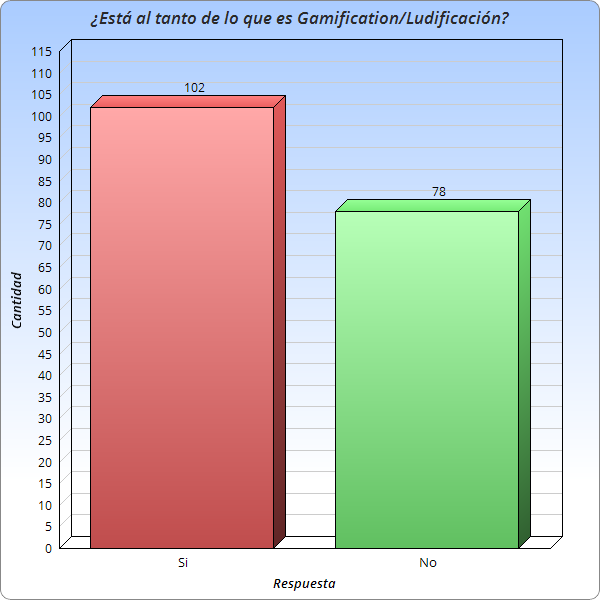
\includegraphics[width=0.6\textwidth]{images/Graficos/graf_5_1.png}
    \caption[chart5.1]{Respuesta a pregunta $3$, conocimiento de {\GAM}.}
    \label{fig:chart5.1}
    %\url{http://www.chartgo.com/get.do?id=69b1dc7d4e}
\end{figure}

La siguiente pregunta,
¿Usted acumula puntos de grandes empresas?, fue creada con el motivo de reforzar
al usuario una forma de {\GAM} con la cual se relaciona frecuentemente y así dar
a entender de mejor forma el concepto.
En esta se obtiene un resultado similar al obtenido en la pregunta anterior,
donde un 56\% contesta positivamente, como la figura  \ref{fig:chart5.2} lo muestra.
Con esta respuesta se ratifica que existe algún conocimiento sobre {\GAM} por parte
mas de la mitad de los encuestados, además se demuestra que han interactuado con
ella de alguna forma.

\begin{figure}[!htb]
    \centering
    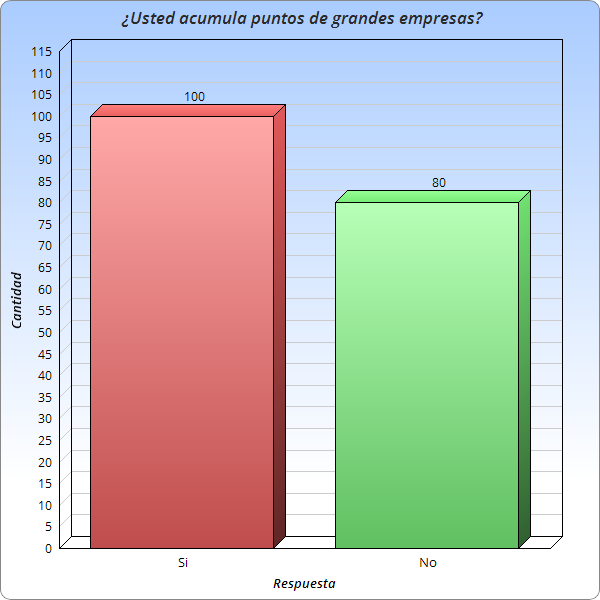
\includegraphics[width=0.6\textwidth]{images/Graficos/graf_5_2.png}
    \caption[chart5.2]{Respuesta a pregunta 4, acumulación de puntos.}
    \label{fig:chart5.2}
    %\url{http://www.chartgo.com/get.do?id=69b1dc7d4e}
\end{figure}

Las preguntas 5 y 6 son exclusivas para las personas que respondieron positivamente
la pregunta anterior (número 4).
Estas preguntas no son obligatorias por lo cual la muestra poblacional
es menor a la obtenida en la encuesta, ambas tienen universos diferentes.
En la primera existen $92$ encuestados que constituyen el 100\%, figura  \ref{fig:chart5.3}.
Esta pregunta tiene como objetivo conocer si los encuestados están en conocimiento
de los beneficios entregados por las empresas.
Con 69 personas contestando positivamente, equivalente a 75\%, se puede apreciar
que los encuestados tienen conocimientos del fin detrás de la acumulación de puntos,
y es esto lo que crea el motivo de volver y seguir comprando en una tienda
\emph{on-line} o presencial.

La siguiente pregunta tiene un universo de 101 personas, figura  \ref{fig:chart5.4},
del cual un 78\% contesto de forma positiva.
Con esto se remarca que los encuestados están en conocimiento de toda la
información necesaria para motivarlos a seguir y conquistar su meta.

\begin{figure}[!htb]
    \centering
    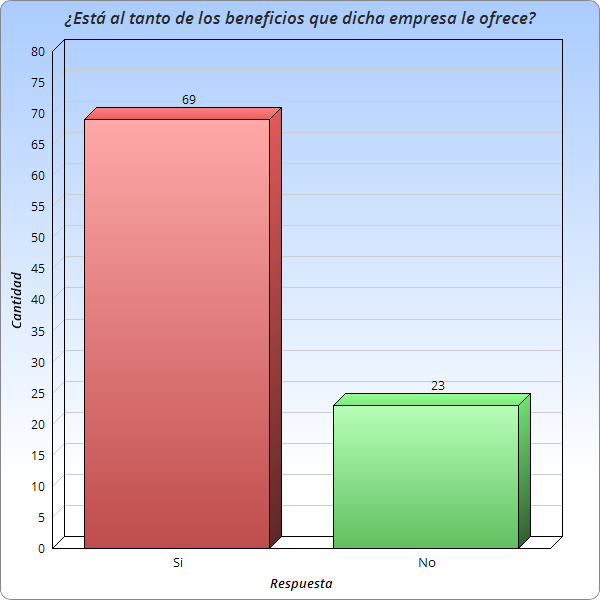
\includegraphics[width=0.6\textwidth]{images/Graficos/graf_5_3.png}
    \caption[chart5.3]{Respuesta a pregunta 5, conocimiento de beneficios.}
    \label{fig:chart5.3}
    %\url{http://www.chartgo.com/get.do?id=69b1dc7d4e}
\end{figure}

\begin{figure}[!htb]
    \centering
    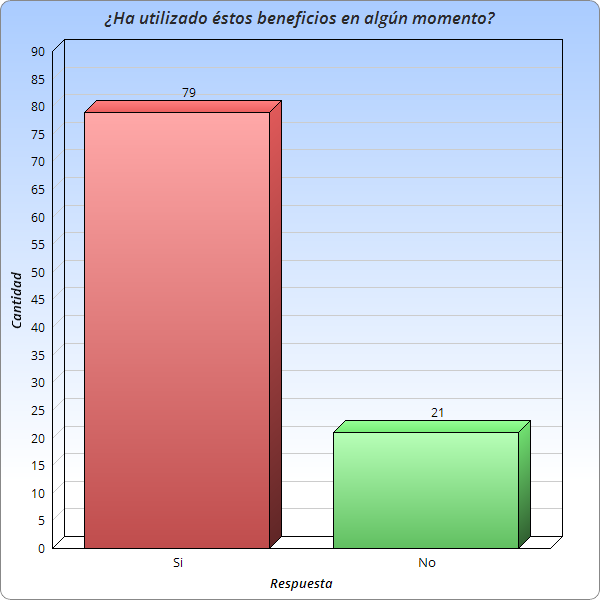
\includegraphics[width=0.6\textwidth]{images/Graficos/graf_5_4.png}
    \caption[chart5.4]{Respuesta a pregunta 6, utilización de los beneficios.}
    \label{fig:chart5.4}
    %\url{http://www.chartgo.com/get.do?id=69b1dc7d4e}
\end{figure}


La siguiente pregunta,
¿Qué beneficios prefiere o preferiría obtener?,
tiene como objetivo conocer los  beneficios mas atractivos para el usuario.
Esta pregunta es del tipo \emph{Likert}\footnote{http://en.wikipedia.org/wiki/Likert\_scale}, 
consta de una escala de preferencia de
1 a 5, siendo 1 la preferencia menos interesante y 5 la más interesante.
El beneficio con mas preferencias 5, o mas interesante para los encuestados,
es la obtención de descuentos en dinero con un 79\%, \ref{fig:chart5.4}.
El siguiente beneficio con mas interesados es la adquisición de descuentos para
próximas compras con un 32\%, figura \ref{fig:chart5.5} de los encuestados.
Una información importante obtenida es que una de las herramientas más utilizadas,
obtención de puntos, es resentida por las personas debido a que existe un mayor
rechazo, 22\%, que aceptación, 18\%, pero la diferencia no es sustantiva para
descartarla como método a utilizar.
El beneficio mas rechazado, mayor cantidad de 1, fue la obtención de un
reconocimiento por tabla de posiciones con un 81\%.

\begin{figure}[!htb]
  \centering
  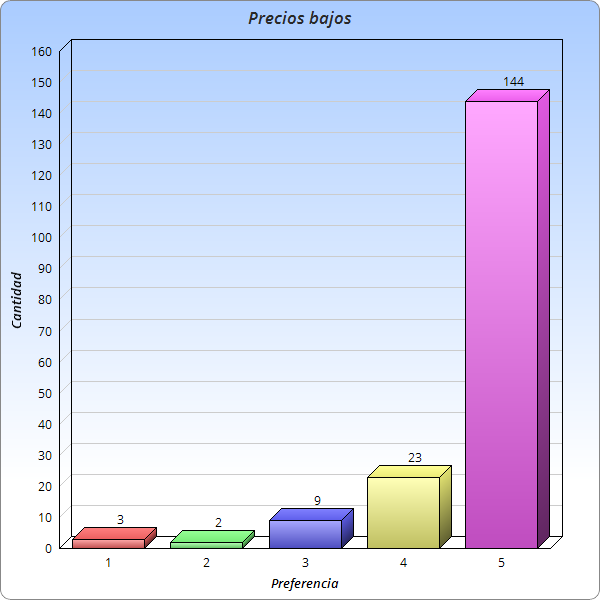
\includegraphics[width=0.6\textwidth]{images/Graficos/graf_5_5.png}
  \caption[chart5.5]{Respuesta a pregunta 7, cantidad de preferencias a beneficio de precios bajos.}
  \label{fig:chart5.5}
  %\url{http://www.chartgo.com/get.do?id=69b1dc7d4e}
\end{figure}

\begin{figure}[!htb]
  \centering
  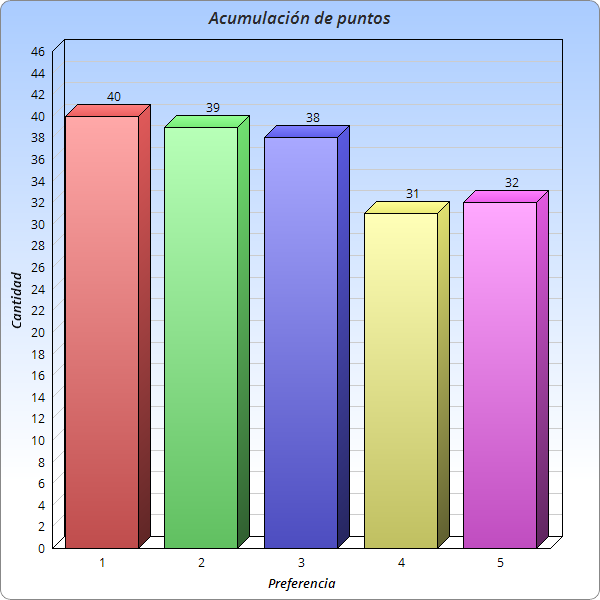
\includegraphics[width=0.6\textwidth]{images/Graficos/graf_5_6.png}
  \caption[chart5.6]{Respuesta a pregunta 7, cantidad de preferencias a beneficio de acumulación de puntos.}
  \label{fig:chart5.6}
  %\url{http://www.chartgo.com/get.do?id=69b1dc7d4e}
\end{figure}

\begin{figure}[!htb]
  \centering
  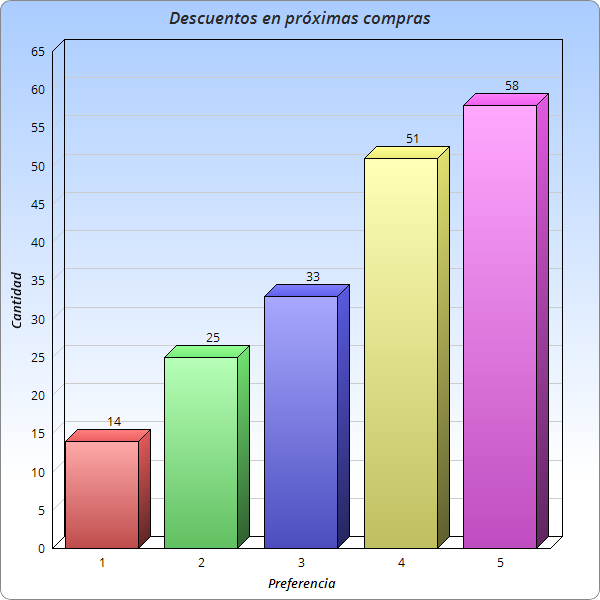
\includegraphics[width=0.6\textwidth]{images/Graficos/graf_5_7.png}
  \caption[chart5.7]{Respuesta a pregunta 7, cantidad de preferencias a beneficio de descuento en
próximas compras.}
  \label{fig:chart5.7}
  %\url{http://www.chartgo.com/get.do?id=69b1dc7d4e}
\end{figure}

\begin{figure}[!htb]
  \centering
  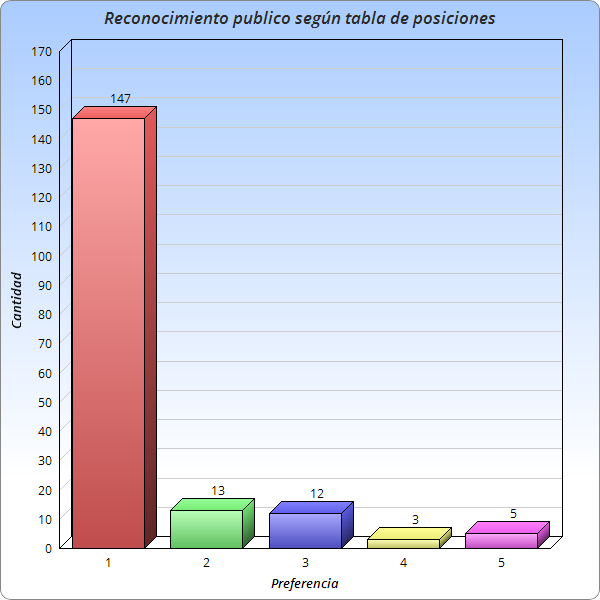
\includegraphics[width=0.6\textwidth]{images/Graficos/graf_5_8.png}
  \caption[chart5.8]{Respuesta a pregunta 7, cantidad de preferencias a beneficio de reconocimiento
publico según tabla de posiciones.}
  \label{fig:chart5.8}
  %\url{http://www.chartgo.com/get.do?id=69b1dc7d4e}
\end{figure}


La pregunta 8,
¿Cuál es su preferencia a la hora de realizar compras?,
muestra cual es la preferencia a la hora de comprar, presencial u \emph{on-line}.
La preferencia mas seleccionada, por 134 personas, fue la opción de compra
presencial.
Esto indica que en Chile no se acostumbra a comprar vía internet y esto representa
una oportunidad de negocio debido al incremento de alfabetización digital y
con esto el aumento del acceso al internet.

\begin{figure}[!htb]
  \centering
  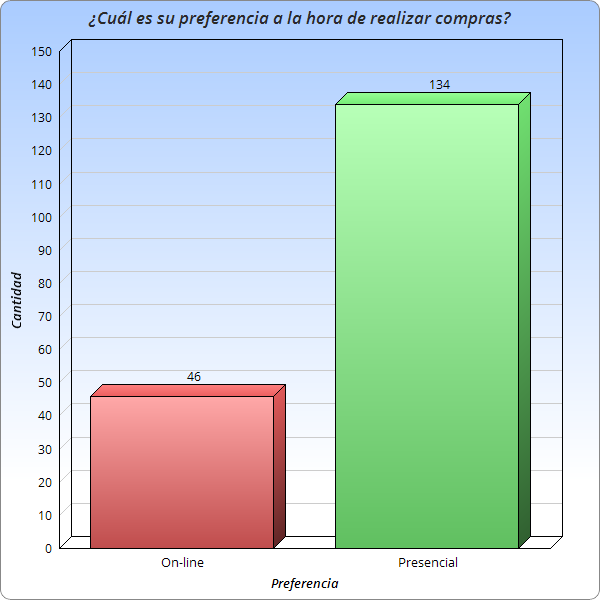
\includegraphics[width=0.6\textwidth]{images/Graficos/graf_5_9.png}
  \caption[chart5.9]{Respuesta a pregunta 8, preferencia al momento de comprar.}
  \label{fig:chart5.9}
  %\url{http://www.chartgo.com/get.do?id=69b1dc7d4e}
\end{figure}

Una vez respondida la pregunta anterior se le expone al usuario, en la pregunta 9,
si preferiría utilizar un sitio de ventas \emph{on-line} convencional, sólo es utilizado
para la transacción entre cliente y empresa, o un sitio el cual ofrezca
herramientas de {\GAM}.
Con un 69\% seleccionan una tienda con {\GAM} como la alternativa preferida.
Con este resultado se remarca la utilización de este concepto con el fin de atraer
a nuevos usuarios.

\begin{figure}[!htb]
  \centering
  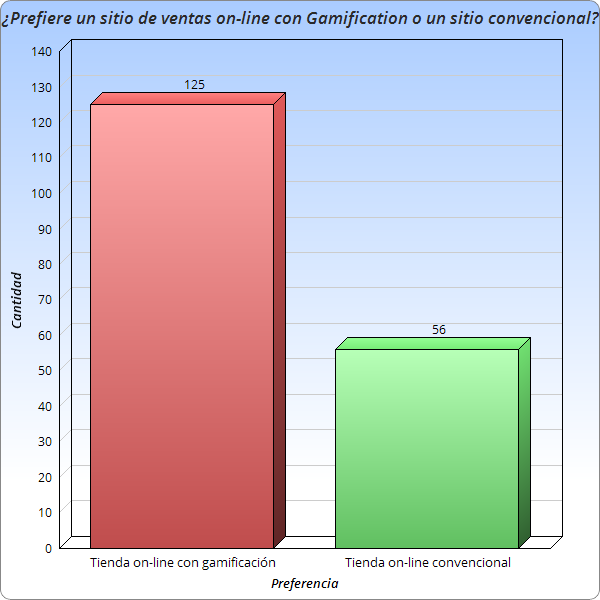
\includegraphics[width=0.6\textwidth]{images/Graficos/graf_5_10.png}
  \caption[chart5.10]{Respuesta a pregunta 9, preferencia al momento de comprar de forma \emph{on-line}.}
  \label{fig:chart5.10}
  %\url{http://www.chartgo.com/get.do?id=69b1dc7d4e}
\end{figure}


La pregunta 10 intenta ratificar una de las mayores ideas tras la utilización
de {\GAM}, la motivación.
Este sentimiento se crea en el usuario con el fin de atraer y retener a este
cliente.
Se obtuvo que 122 personas han creado este sentimiento que los impulsa a volver
a utilizar o comprar en la tienda implementada con {\GAM}.
Esta información es bastante importante al momento de implementar una solución
gamificada y aun mas cuando se trata de comercio electrónico.

\begin{figure}[!htb]
  \centering
  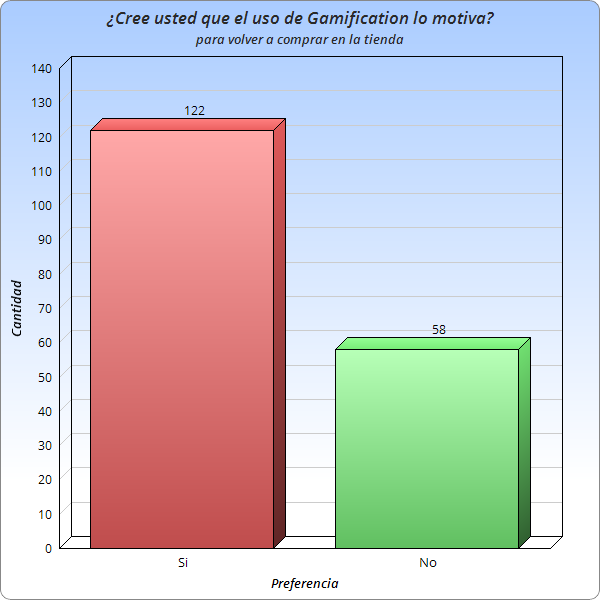
\includegraphics[width=0.6\textwidth]{images/Graficos/graf_5_11.png}
  \caption[chart5.11]{Respuesta a pregunta 10, motivación para volver a comprar en una misma tienda.}
  \label{fig:chart5.11}
  %\url{http://www.chartgo.com/get.do?id=69b1dc7d4e}
\end{figure}

Por último,
se intenta obtener una idea de que contextos podrían ser interesantes para
implementar una solución gamificada.
Con esto en mente, la más votada fue el contexto social con 109 preferencias,
seguida por educación con 100 encuestados.
Con esta información se pueden inferir ideas para desarrollos futuros en esta área.

\begin{figure}[!htb]
  \centering
  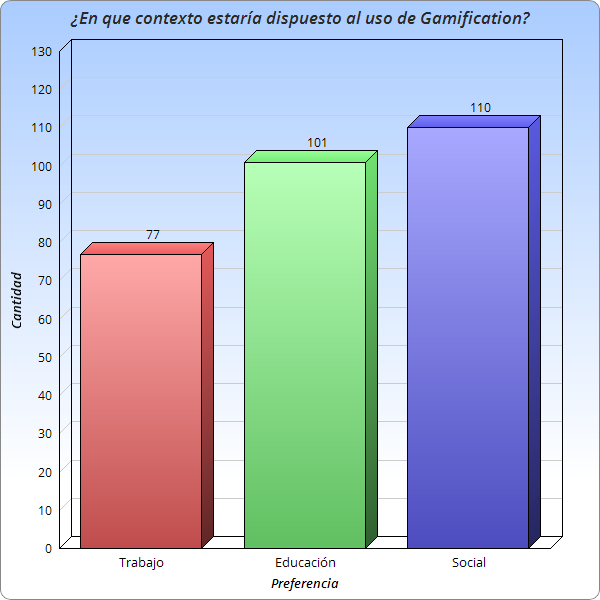
\includegraphics[width=0.6\textwidth]{images/Graficos/graf_5_12.png}
  \caption[chart5.12]{Respuesta a pregunta 11, contextos a los cuales se le podría implementar {\GAM}.}
  \label{fig:chart5.12}
  %\url{http://www.chartgo.com/get.do?id=69b1dc7d4e}
\end{figure}

Luego de realizar la implementación {\GAM} sobre una tienda \emph{on-line} y con los datos
obtenidos mediante la encuesta realizada se obtuvo bastante información para
analizar y obtener conclusiones que ayudaran a futuras empresas que quieran
utilizar este concepto en sus empresas. También se obtiene información para guiar
trabajos futuros en otros contextos.

\begin{table}[h]
\footnotesize
\setlength\extrarowheight{5pt}
\begin{tabular}{| p{4cm} | p{1.8cm} | p{2.5cm} | p{2.8cm} |}
\hline
                          Pregunta
                        & Porcentaje \newline Si
                        & Porcentaje \newline No
                        & Total \newline preferencias \\ \hline
¿Está al tanto de lo que es {\gam} - ludificación?&1&1&1 \\
\end{tabular}
\caption{Tabla de comparación entre los sistemas bases investigados}
\label{tab:comp_tools}
\end{table}


\chapter{Conclusiones}
\label{ch:conclusiones}
    El presente trabajo de memoria aborda la problemática que poseen las pequeñas
empresas al tratar de competir con empresas de mayor tamaño, mayor capital
económico o humano, en lo que a ventas se refiere. Esto mediante la utilización de {\gam} 
como herramienta para atraer y retener clientes con el propósito de incrementar las ventas.

\section{Objetivos cumplidos}

Analizando los datos obtenidos en el capítulo \ref{ch:estudio}, se puede observar que el
implementar un sitio base nuevo, para una micro o pequeña empresa, con todas las
herramientas de venta de artículos \emph{on-line}, además introducir el concepto de {\gam} en el sistema,
 es una tarea bastante compleja.

Para implementar de forma exitosa el sistema completo, se necesitan ciertos factores
complementarios como son el interés de la empresa, estabilidad económica de ésta y la necesidad del cliente 
por utilizar el sistema. Es importante, una vez implementado el sistema, que no existan restricciones 
al utilizar los puntos canjeables, una limitación en esto es perjudicial y disminuye la motivación del 
cliente para volver a la tienda.
También es de utilidad, que al momento de la implementación, se realice publicidad
de la tienda para aumentar el número de visitas y así mostrar las nuevas herramientas. 
Por último, es recomendable utilizar medios de pago que sean conocidos
por los clientes con el objetivo de crear un sentimiento de seguridad en ellos, este factor es importante
ya que la transacción es el paso final entre empresa y cliente.

Por otra parte, luego de analizar los datos obtenidos en la encuesta, en el capítulo \ref{ch:estudio},
 se puede observar que {\gam} es un concepto bastante conocido y utilizado por las personas
entre 18 y 32 años, debido a que son usuarios de las herramientas de {\gam} entregadas por
diferentes empresas(puntos, recompensas, etc), y que a su vez lo hacen con el fin de utilizar los beneficios entregados
por éstas. El beneficio más interesante para el cliente es el obtener descuentos en dinero
que pudiesen ser utilizados de forma inmediata o para próximas compras.

En cuanto a la forma de entrega de beneficios más utilizada en el mercado es el intercambio de puntos.
Al analizar este punto con lo obtenido en la encuesta se puede determinar que no es
una opción interesante para el cliente y que se debería investigar otra forma para
hacer entrega de los beneficios. Una alternativa en la entrega de beneficios fijos por nivel
de usuario, tipos de usuarios,  y que estos sean otorgados mediante el número de compras o achievements logrados
dentro de la tienda.

Gracias a la información obtenida de la encuesta, se confirma la
idea principal de {\gam}, la cual es utilizar la motivación como herramienta para
que el usuario sienta la necesidad de volver a utilizar el sistema y
se espera que una solución, a cualquier problemática, implementando {\gam} se
enfoque sobre esta idea.

\section{{\GAM} en Chile}

Si bien en Chile el concepto de {\gam} es utilizado hace tiempo por empresas de gran tamaño, no se
puede decir lo mismo para aquellas pequeñas empresas. Para que una de estas empresas pueda
llegar a utilizar la idea de {\gam},ésta se debe hacer asesorar por especialistas, lo cual
requiere recursos, tales como monetarios y de tiempo, que no pueden destinar a mejorar su interacción con el usuario.

Luego de realizar éste trabajo de memoria se puede observar que la utilización de {\gam} en Chile tiene
un gran impacto en la interacción entre empresa y usuario debido a que estos últimos reconocen el uso
periódico de las herramientas que entrega {\gam}, como se mencionó antes.
En esta investigación se realizo una encuesta que apoya directamente el uso de {\gam} en las tienda, tanto
on-line como establecidas, debido a que el usuario chileno necesita del estimulo que obtiene, beneficios o productos,
al momento de elegir el lugar donde realizara sus compras. Tomando ésta información se ve necesario que las
pequeñas empresas de Chile tomen el concepto de {\gam} como una herramienta para poder competir con sus
pares que ya utilizan {\gam} y ven los beneficios de este concepto diariamente.

Una vez analizada toda la información obtenida se puede concluir que {\gam} es un concepto que influye
en el usuario del país y que el sistema propuesto para incorporar {\gam} en la pequeña empresa
es una herramienta importante y que debería ayudar, en el mediano a largo plazo, a competir con empresas
de mayor tamaño en lo que tiendas virtuales se refiere.

\section{Herramientas}

Una parte importante del sistema propuesto como solución son las herramientas utilizadas para su creación.
La primera herramienta requerida fue el sistema base, \emph{Wordpress + Woocommerce}, el cual luego de
la implementación demostró ser la mejor opción para ser enfocada en la pequeña empresa debido a su
fácil administración y baja curva de aprendizaje para los nuevos usuarios. Las otra opciones para sistema no lograron
destacar en las características necesarias para ser consideradas en esta implementación pero deben ser
tomadas en consideración cuando se desee implementar un sistema para empresas de mayor tamaño.

Las demás herramientas, \emph{WooCube Pro}, \emph{WPAchievement} y \emph{Refer a Friend}, utilizadas en la 
implementación entregan las funcionalidades necesarias para mostrar las ideas de {\gam} en la tienda virtual. Estas funcionalidades son la acumulación de puntos, referir a un amigo o medallas por logros realizados. Otra característica por
lo cual fueron seleccionadas es el soporte con el cual cuentan y que el costo de estas es bajo.

Si bien cada una de estas herramientas fue desarrollada por una empresa diferente, se logró una excelente
integración entre ellas lo cual facilito la implementación al no necesitar un modulo que ayudara en la comunicación
entre estas herramientas.

Finalmente, con las herramientas seleccionadas se logro realizar una implementación exitosa y se espera que para
el uso en una pequeña empresa no sea necesario añadir nuevas herramientas.

\section{Cliente}

Para la implementación de la solución propuesta se contó con la ayuda de ``Kurgan Juegos''. Una vez terminada
la recolección de datos y con la información obtenida de esto, capítulo \ref{cap_estudio}, se le comunico
al cliente los problemas obtenidos en esta etapa, no logrando un registro o venta, con el objetivo de obtener
sus pensamientos al respecto.

Si bien no se logro realizar un registro de usuario o venta a través de la tienda el cliente quedo conforme con
el sitio tomando en consideración el alza de visitas que presento la web. También explico la baja de motivación,
del cliente, en la utilización del sistema. Uno de los factores fue el momento económico en el cual estaba la tienda
el cual no ayudo al momento de presentar una gran cantidad de productos en la tienda virtual. Otro factor, fue la
mala organización del stock de productos en la tienda el cual fue problema al momento de agregar los productos
a la tienda virtual.

Finalmente, el cliente quedo conforme con el resultado general del sistema aun así no logrando una gran aceptación 
de esta debido a los factores antes descritos.

\subsection{Trabajos futuros}

En ésta investigación se proponen las siguientes ideas como trabajos futuros:


\begin{itemize}

\item Realizar una adecuada publicidad sobre el sistema nuevo implementado para
	atraer más clientes a conocer la nueva tienda on-line. Además analizar
	la población interesada y mejorar el sistema implementando técnicas
	enfocadas a esta población.

\item El sistema base utilizado en este trabajo de memoria, Wordpress $+$ Woocommerce, contiene
todo lo necesario para ser utilizado por micro o pequeñas empresas, la escalabilidad está limitada
a la compra de plugins. En el capítulo 4, tabla \ref{tab:comp_tools}, se analizaron dos sistemas más
que podrían ser útiles si se requiere implementar {\GAM} en tiendas de mayor tamaño, ya que contienen
más utilidades incorporadas en el mismo sistema base, en especial \emph{Magento}.

\item Investigar y utilizar otra forma de entrega de beneficios, debido a que la
acumulación de puntos no es bastante interesante para la población. Una nueva forma podría ser la entrega
de beneficios fijo por nivel de cliente y por la cantidad de logros obtenidos.

\end{itemize}




\singlespacing
\bibliographystyle{plain}
\bibliography{references}

\chapter{Anexos}
\label{ch:anexos}
    \section{Anexo I: Encuesta evaluativa}
\label{AnexoI}
\begin{enumerate}

\item ¿Sexo?: \\

$\bigcirc$ Masculino \\
$\bigcirc$ Femenino

\item Rango de edad: \\

$\bigcirc 10 - 17$\\
$\bigcirc 18 - 24$\\
$\bigcirc 25 - 32$\\
$\bigcirc 33 - 39$\\
$\bigcirc 40 - $o más

\item ¿Está al tanto de lo que es ``{\gam}/ludificación'' ? \\

$\bigcirc$ Si \\
$\bigcirc$ No

\item ¿Usted acumula puntos de grandes empresas?\\

$\bigcirc$ Si \\
$\bigcirc$ No    

\item  (Si contesto ``No'' en la pregunta anterior, pasar a la pregunta 7.) En empresas donde sea socio o participe acumulando puntos, ¿Está al tanto de los beneficios que dicha empresa le ofrece?\\

$\bigcirc$ Si \\
$\bigcirc$ No

\item ¿Ha utilizado éstos beneficios en algún momento?\\

$\bigcirc$ Si \\
$\bigcirc$ No

\item Al momento de comprar, ¿Qué beneficios prefiere o preferiría obtener?:

\begin{table}[h]
\centering
\begin{tabular}{|l|c|c|c|c|c|}
\hline
 & {\bf 1} & {\bf 2} & {\bf 3} & {\bf 4} & {\bf 5} \\
\hline
Precios bajos. & $\bigcirc$ & $\bigcirc$ & $\bigcirc$ & $\bigcirc$ & $\bigcirc$ \\
\hline
Acumulación de puntos. & $\bigcirc$ & $\bigcirc$ & $\bigcirc$ & $\bigcirc$ & $\bigcirc$ \\
\hline
Descuentos en próximas compras. & $\bigcirc$ & $\bigcirc$ & $\bigcirc$ & $\bigcirc$ & $\bigcirc$ \\
\hline
Obtención de productos exclusivos. & $\bigcirc$ & $\bigcirc$ & $\bigcirc$ & $\bigcirc$ & $\bigcirc$ \\
\hline
Reconocimiento publico según tabla de posiciones. & $\bigcirc$ & $\bigcirc$ & $\bigcirc$ & $\bigcirc$ & $\bigcirc$ \\
\hline
\end{tabular}
\end{table}

\item ¿Cuál es su preferencia a la hora de realizar compras? \\

$\bigcirc$ Presencial (persona a persona) \\
$\bigcirc$ On-line (vía internet)

\item Teniendo en cuenta lo que consiste ``{\gam}'', ¿Prefiere un sitio de ventas on-line con ``{\gam}'' o un sitio convencional? \\

$\bigcirc$ Tienda on-line con {\gam} \\
$\bigcirc$ Tienda on-line convencional

\item ¿Cree usted que el uso de ``{\gam}'' lo motiva para volver a comprar en la tienda? \\

$\bigcirc$ Si \\
$\bigcirc$ No

\item  ¿En que contexto estaría dispuesto al uso de ``{\gam}''?(Puede responder más de una)\\
 
$\bigcirc$ Trabajo. Ej. Reconocimiento y motivación mediante el uso de una tabla de posiciones asociada a la productividad. \\
$\bigcirc$ Educación. Ej: Entrega de beneficios por tareas completadas. Estos beneficios pueden ser la utilización de puntos para poder cambiar preguntas de una prueba por otra. \\
$\bigcirc$  Social. Ej: Conectar con personas para obtener beneficios mutuos. Un tipo de beneficios es descuentos al invitado y al que hizo la invitación luego de la primera compra del invitado.
\end{enumerate}

\section{Anexo II: Gráficos }

\begin{figure}[!htb]
    \centering
    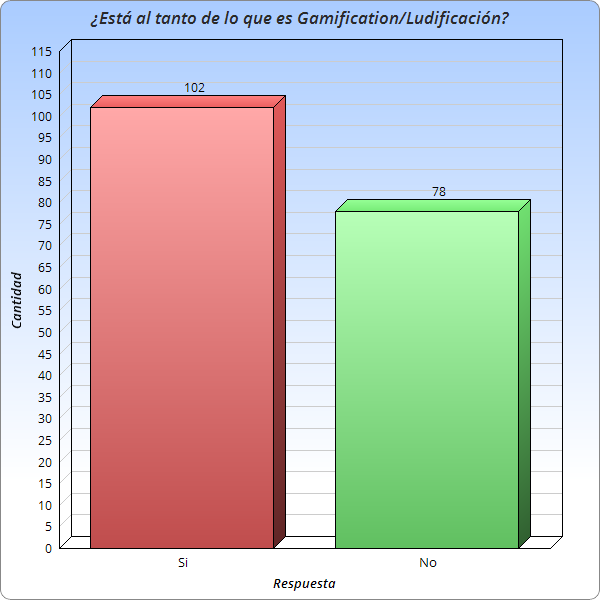
\includegraphics[width=0.6\textwidth]{images/Graficos/graf_5_1.png}
    \caption[Gráfico pregunta 3 de encuesta, conocimiento de {\gam}.]{Respuesta a pregunta $3$, conocimiento de {\gam}.}
    \label{fig:chart5.1}
    %\url{http://www.chartgo.com/get.do?id=69b1dc7d4e}
\end{figure}

\begin{figure}[!htb]
    \centering
    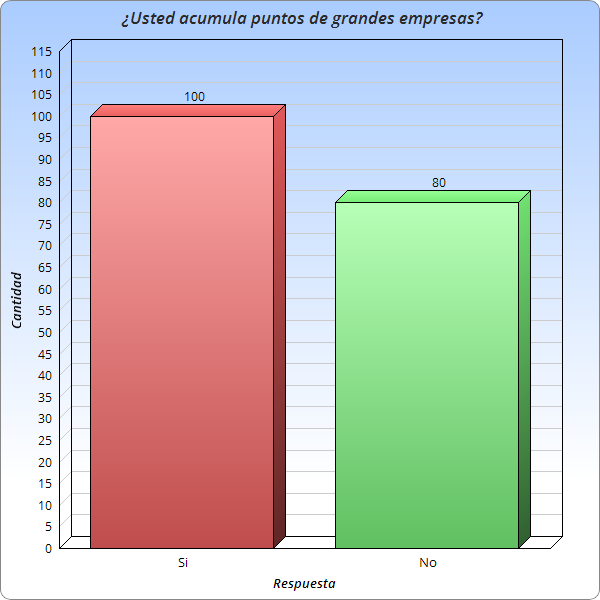
\includegraphics[width=0.6\textwidth]{images/Graficos/graf_5_2.png}
    \caption[Gráfico pregunta 4, acumulación de puntos.]{Respuesta a pregunta 4, acumulación de puntos.}
    \label{fig:chart5.2}
    %\url{http://www.chartgo.com/get.do?id=69b1dc7d4e}
\end{figure}

\begin{figure}[!htb]
    \centering
    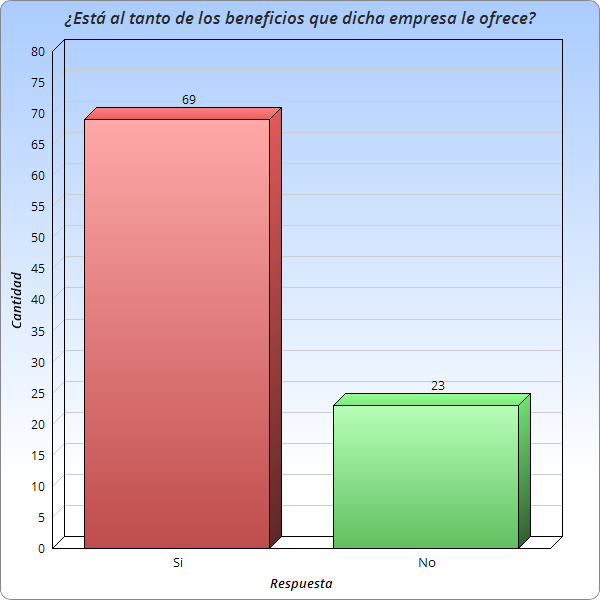
\includegraphics[width=0.6\textwidth]{images/Graficos/graf_5_3.png}
    \caption[Gráfico pregunta 5, conocimiento de beneficios.]{Respuesta a pregunta 5, conocimiento de beneficios.}
    \label{fig:chart5.3}
    %\url{http://www.chartgo.com/get.do?id=69b1dc7d4e}
\end{figure}

\begin{figure}[!htb]
    \centering
    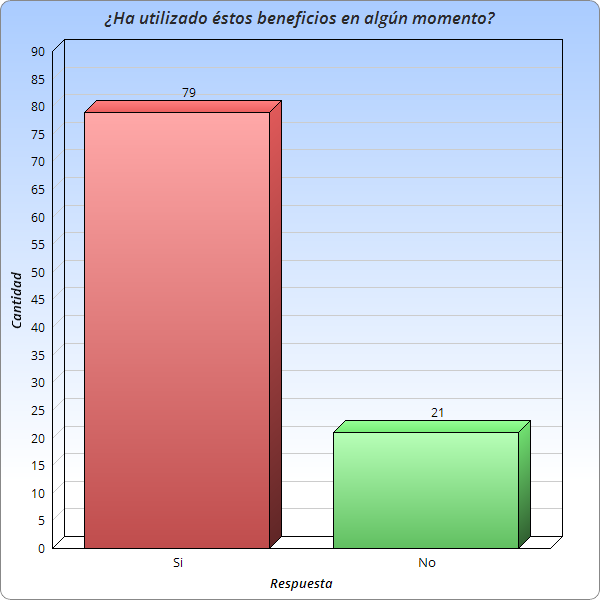
\includegraphics[width=0.6\textwidth]{images/Graficos/graf_5_4.png}
    \caption[Gráfico pregunta 6, utilización de los beneficios.]{Respuesta a pregunta 6, utilización de los beneficios.}
    \label{fig:chart5.4}
    %\url{http://www.chartgo.com/get.do?id=69b1dc7d4e}
\end{figure}

\begin{figure}[!htb]
  \centering
  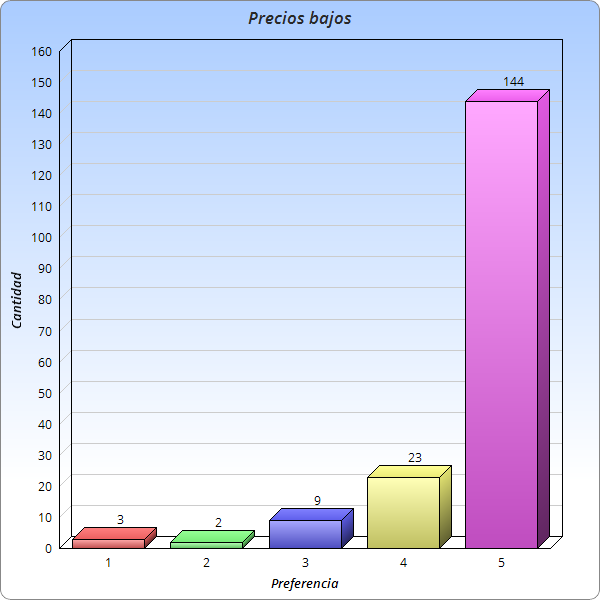
\includegraphics[width=0.6\textwidth]{images/Graficos/graf_5_5.png}
  \caption[Gráfico pregunta 7, cantidad de preferencias a beneficio de precios bajos.]{Respuesta a pregunta 7, cantidad de preferencias a beneficio de precios bajos.}
  \label{fig:chart5.5}
  %\url{http://www.chartgo.com/get.do?id=69b1dc7d4e}
\end{figure}

\begin{figure}[!htb]
  \centering
  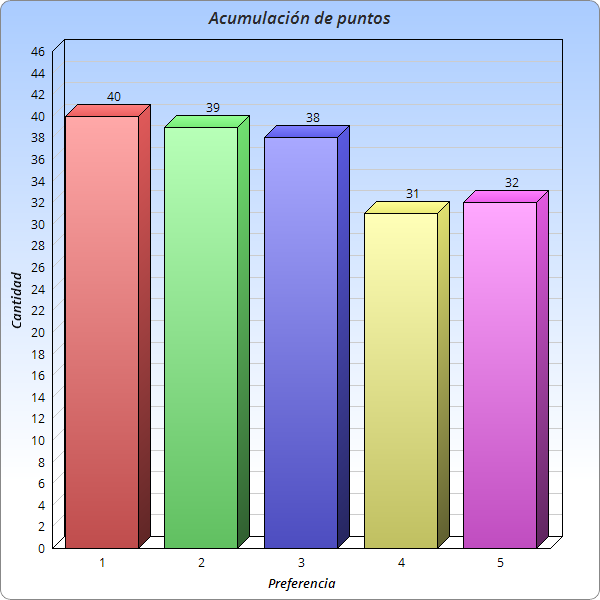
\includegraphics[width=0.6\textwidth]{images/Graficos/graf_5_6.png}
  \caption[Gráfico pregunta 7, cantidad de preferencias a beneficio de acumulación de puntos.]{Respuesta a pregunta 7, cantidad de preferencias a beneficio de acumulación de puntos.}
  \label{fig:chart5.6}
  %\url{http://www.chartgo.com/get.do?id=69b1dc7d4e}
\end{figure}

\begin{figure}[!htb]
  \centering
  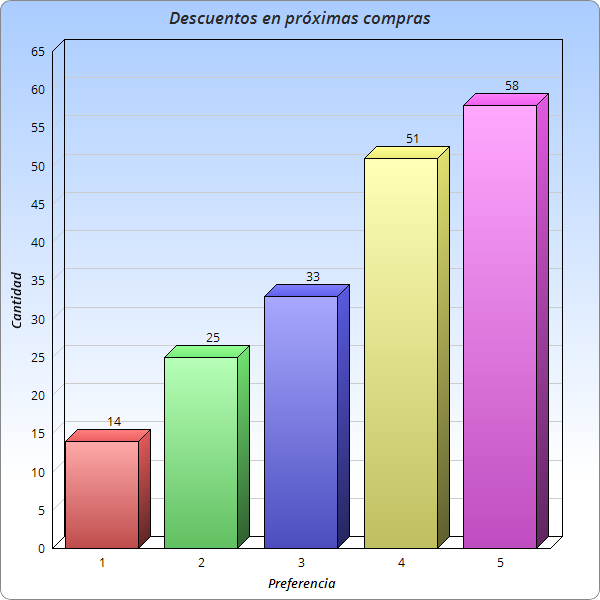
\includegraphics[width=0.6\textwidth]{images/Graficos/graf_5_7.png}
  \caption[Gráfico pregunta 7, cantidad de preferencias a beneficio de descuento en
próximas compras.]{Respuesta a pregunta 7, cantidad de preferencias a beneficio de descuento en
próximas compras.}
  \label{fig:chart5.7}
  %\url{http://www.chartgo.com/get.do?id=69b1dc7d4e}
\end{figure}

\begin{figure}[!htb]
  \centering
  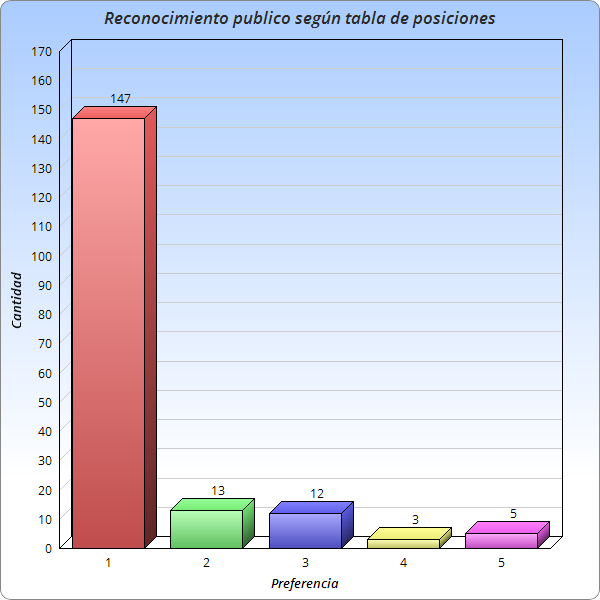
\includegraphics[width=0.6\textwidth]{images/Graficos/graf_5_8.png}
  \caption[Gráfico pregunta 7, cantidad de preferencias a beneficio de reconocimiento
publico según tabla de posiciones.]{Respuesta a pregunta 7, cantidad de preferencias a beneficio de reconocimiento
publico según tabla de posiciones.}
  \label{fig:chart5.8}
  %\url{http://www.chartgo.com/get.do?id=69b1dc7d4e}
\end{figure}

\begin{figure}[!htb]
  \centering
  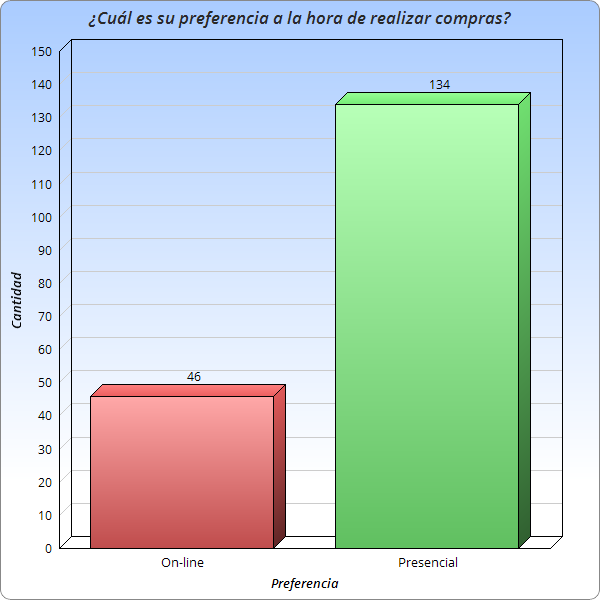
\includegraphics[width=0.6\textwidth]{images/Graficos/graf_5_9.png}
  \caption[Gráfico pregunta 8, preferencia al momento de comprar.]{Respuesta a pregunta 8, preferencia al momento de comprar.}
  \label{fig:chart5.9}
  %\url{http://www.chartgo.com/get.do?id=69b1dc7d4e}
\end{figure}

\begin{figure}[!htb]
  \centering
  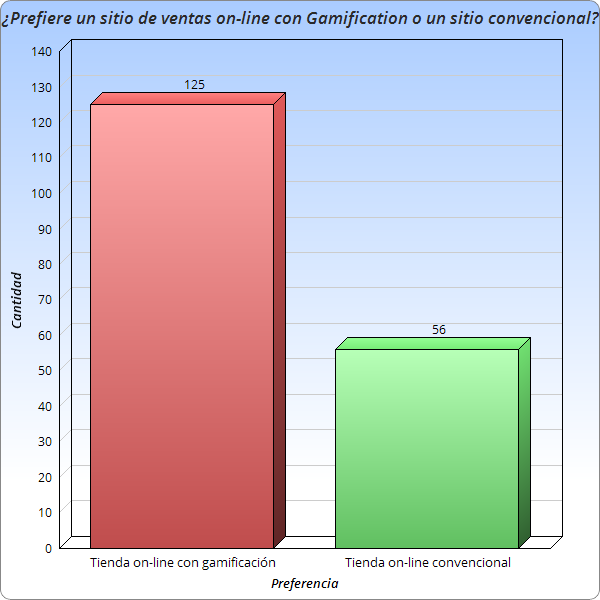
\includegraphics[width=0.6\textwidth]{images/Graficos/graf_5_10.png}
  \caption[Gráfico pregunta 9, preferencia al momento de comprar de forma \emph{on-line}.]{Respuesta a pregunta 9, preferencia al momento de comprar de forma \emph{on-line}.}
  \label{fig:chart5.10}
  %\url{http://www.chartgo.com/get.do?id=69b1dc7d4e}
\end{figure}

\begin{figure}[!htb]
  \centering
  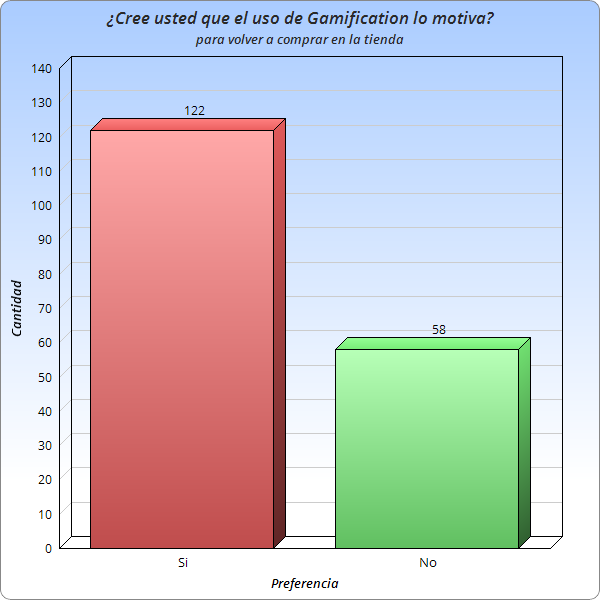
\includegraphics[width=0.6\textwidth]{images/Graficos/graf_5_11.png}
  \caption[Gráfico pregunta 10, motivación para volver a comprar en una misma tienda.]{Respuesta a pregunta 10, motivación para volver a comprar en una misma tienda.}
  \label{fig:chart5.11}
  %\url{http://www.chartgo.com/get.do?id=69b1dc7d4e}
\end{figure}

\begin{figure}[!htb]
  \centering
  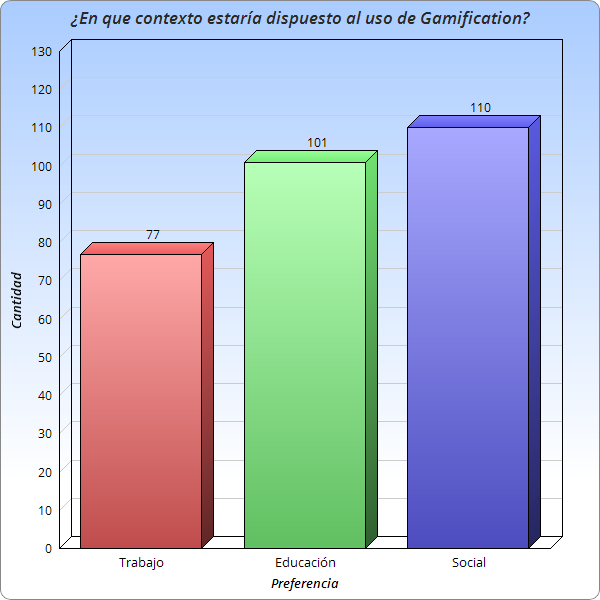
\includegraphics[width=0.6\textwidth]{images/Graficos/graf_5_12.png}
  \caption[Gráfico pregunta 11, contextos a los cuales se le podría implementar {\gam}.]{Respuesta a pregunta 11, contextos a los cuales se le podría implementar {\gam}.}
  \label{fig:chart5.12}
  %\url{http://www.chartgo.com/get.do?id=69b1dc7d4e}
\end{figure}



\end{document}

